\documentclass[12pt,]{article}
\usepackage{lmodern}
\usepackage{amssymb,amsmath}
\usepackage{ifxetex,ifluatex}
\usepackage{fixltx2e} % provides \textsubscript
\ifnum 0\ifxetex 1\fi\ifluatex 1\fi=0 % if pdftex
  \usepackage[T1]{fontenc}
  \usepackage[utf8]{inputenc}
\else % if luatex or xelatex
  \ifxetex
    \usepackage{mathspec}
    \usepackage{xltxtra,xunicode}
  \else
    \usepackage{fontspec}
  \fi
  \defaultfontfeatures{Mapping=tex-text,Scale=MatchLowercase}
  \newcommand{\euro}{€}
\fi
% use upquote if available, for straight quotes in verbatim environments
\IfFileExists{upquote.sty}{\usepackage{upquote}}{}
% use microtype if available
\IfFileExists{microtype.sty}{%
\usepackage{microtype}
\UseMicrotypeSet[protrusion]{basicmath} % disable protrusion for tt fonts
}{}
\usepackage[margin=1in]{geometry}
\usepackage{graphicx}
\makeatletter
\def\maxwidth{\ifdim\Gin@nat@width>\linewidth\linewidth\else\Gin@nat@width\fi}
\def\maxheight{\ifdim\Gin@nat@height>\textheight\textheight\else\Gin@nat@height\fi}
\makeatother
% Scale images if necessary, so that they will not overflow the page
% margins by default, and it is still possible to overwrite the defaults
% using explicit options in \includegraphics[width, height, ...]{}
\setkeys{Gin}{width=\maxwidth,height=\maxheight,keepaspectratio}
\ifxetex
  \usepackage[setpagesize=false, % page size defined by xetex
              unicode=false, % unicode breaks when used with xetex
              xetex]{hyperref}
\else
  \usepackage[unicode=true]{hyperref}
\fi
\hypersetup{breaklinks=true,
            bookmarks=true,
            pdfauthor={Melissa Monk},
            pdftitle={Workshop Examples},
            colorlinks=true,
            citecolor=blue,
            urlcolor=blue,
            linkcolor=magenta,
            pdfborder={0 0 0}}
\urlstyle{same}  % don't use monospace font for urls
\setlength{\parindent}{0pt}
\setlength{\parskip}{6pt plus 2pt minus 1pt}
\setlength{\emergencystretch}{3em}  % prevent overfull lines
\setcounter{secnumdepth}{5}

%%% Use protect on footnotes to avoid problems with footnotes in titles
\let\rmarkdownfootnote\footnote%
\def\footnote{\protect\rmarkdownfootnote}

%%% Change title format to be more compact
\usepackage{titling}

% Create subtitle command for use in maketitle
\newcommand{\subtitle}[1]{
  \posttitle{
    \begin{center}\large#1\end{center}
    }
}

\setlength{\droptitle}{-2em}
  \title{Workshop Examples}
  \pretitle{\vspace{\droptitle}\centering\huge}
  \posttitle{\par}
  \author{Melissa Monk}
  \preauthor{\centering\large\emph}
  \postauthor{\par}
  \date{}
  \predate{}\postdate{}

% This file contains all of the LaTeX packages you may need to compile the document
% Documentation for each package can be found onlines
\usepackage{tabularx}                                             % table environment providing flexibility
\usepackage{caption}                                              % for creating captions  
\usepackage{longtable}                                            % allows tables to span multiple pages
\usepackage{rotating}                                             % allows for sideways tables
\usepackage{float}                                                % floating environments; may not need in rmarkdown
\usepackage{placeins}                                             % keeps floats from moving
\usepackage{indentfirst}                                          % indents first paragraph of a section
\usepackage{mdwtab}                                               % continued float multi-page figure
\usepackage{enumerate}                                            % create lists
\usepackage{hyperref}                                             % highlight cross references
\hypersetup{colorlinks=true, urlcolor=blue, linktoc=page, linkcolor=blue, citecolor=blue} %define referencing colors
%\usepackage{makebox}                                             % make boxes around text
\usepackage[usenames,dvipsnames]{xcolor}                          % color name options
%\usepackage[space]{grffile}                                      % spaces in file name path
\usepackage{soul}                                                 % highlight text
\usepackage{enumitem}                                             % numbered lists
\usepackage{lineno}                                               % Line numbers; comment out for final
\usepackage{upquote}                                              % produce grave accent in latex
\usepackage{verbatim}                                             % produces verbatim results
\usepackage{fancyvrb}                                             % verbatim in a box
\usepackage[inline]{showlabels}                                   % show table and figure labels; comment out for final
%\usepackage{draftwatermark}                                      % places Draft watermark in background; comment out for final
\usepackage{textcomp}                                             % fixes error with packages interfering
\usepackage{lscape}                                               % rotate pages - to allow for landscape longtables
%\pdfinterwordspaceon                                              % fix loss of inter word spacing
\usepackage{cmap}                                                 % fix mapping characters to unicode
\RequirePackage[linewidth = 1]{pdfcomment}                        %pdf comments
\RequirePackage[l2tabu, orthodox]{nag}                            %checks packages related to the accessibility?
%\RequirePackage[tagged]{accessibilityMeta}

\linenumbers                                                      % specify use of line numbers

\definecolor{light-gray}{gray}{.85}
%\usepackage[tagged]{accessibility-meta}

\begin{document}

\maketitle


{
\hypersetup{linkcolor=black}
\setcounter{tocdepth}{4}
\tableofcontents
}
Change some of the YAML settings to see what happens.

Notice, the down arrow at line 25. If you click this, you can hide the R
code chunk. This is helpful when working through a large document.

On the right side of the R code chunk are additional options, Settings,
a down arrow (run previous R code chunks), and a green play button (runs
the current chunk). It's handy to check R code chunks as you go and to
debug. Within the Assessment template, this is also the only way to see
variables in your Environment.

\section{Emphasis (R markdown and
LaTeX)}\label{emphasis-r-markdown-and-latex}

\emph{Sebastes} \emph{melanops}\\\emph{Sebastes melanops}

<<<<<<< HEAD
\textbf{Sebastes}\\\textbf{\emph{Sebastes}}\\\textbf{Sebastes melanops}\\\emph{\textbf{Sebastes melanops}}

\section*{Headers}\label{headers}
\addcontentsline{toc}{section}{Headers}

\subsection{Subhead 2}\label{subhead-2}

\subsubsection*{Subhead 3}\label{subhead-3}
\addcontentsline{toc}{subsubsection}{Subhead 3}

\paragraph{Subhead 4}\label{subhead-4}
=======
\emph{Sebastes}\\
\emph{Sebastes}

\emph{Sebastes}

\textbf{\emph{Sebastes}}\\
\textbf{Sebastes}\\
\emph{\textbf{Sebastes}}

\section{Headers}\label{headers}
>>>>>>> refs/remotes/melmonk/master

\subsection{Subhead 2}\label{subhead-2}

\subsubsection{Subhead 3}\label{subhead-3}

\paragraph{Subhead 4}\label{subhead-4}

\emph{Subhead 5}

\section{Commenting}\label{commenting}

\section{Links}\label{links}

\href{www.github.com}{Github}

\section{Lists}\label{lists}

<<<<<<< HEAD
R Markdown are finicky with spacing\ldots{} * Item 1 * Item 2 + Item 2a
+ Item 2b

\begin{itemize}
\itemsep1pt\parskip0pt\parsep0pt
=======
R Markdown are finicky with spacing\ldots{}

\begin{itemize}
\tightlist
>>>>>>> refs/remotes/melmonk/master
\item
  Item 1
\item
  Item 2
<<<<<<< HEAD
\item
  Item 2a
\item
  Item 2b
=======

  \begin{itemize}
  \tightlist
  \item
    Item 2a
  \item
    Item 2b
  \end{itemize}
\item
  Item 1
\item
  Item 2

  \begin{itemize}
  \tightlist
  \item
    Item 2a
  \item
    Item 2b
  \end{itemize}
>>>>>>> refs/remotes/melmonk/master
\end{itemize}

Bulleted list

\begin{itemize}[noitemsep,nolistsep,topsep=0pt]

\item \href{https://git-scm.com/book/en/v2/Getting-Started-Installing-Git}{Git}

\item \href{https://cran.r-project.org/bin/windows/base/}{R}

\end{itemize}

Numbered list

\begin{enumerate}[noitemsep,nolistsep,topsep=0pt]

\item \href{https://git-scm.com/book/en/v2/Getting-Started-Installing-Git}{Git}

\item \href{https://cran.r-project.org/bin/windows/base/}{R} 

\end{enumerate}

\section{References and Citations}\label{references-and-citations}

We can reference a document section, see Lists in Section \ref{lists}.

<<<<<<< HEAD
Citations: (Love et al. 2002) Love (2002)
=======
Citations: (Love et al. \protect\hyperlink{ref-Love2002}{2002},
\protect\hyperlink{ref-Love2002}{2002})

Love (\protect\hyperlink{ref-Love2002}{2002})
>>>>>>> refs/remotes/melmonk/master

\section{Figure from a file}\label{figure-from-a-file}

You can use any file extension, including PDFs

\begin{figure}[htbp]
\centering
\includegraphics{RMarkdownFLow.png}
\caption{Here's my caption 1\label{fig:fig_example1}}
\end{figure}

\begin{figure}[htbp]
\centering
\includegraphics{./Figures/RMarkdownFLow1.png}
<<<<<<< HEAD
\caption{Here's my caption 2\label{fig:fig_example2}}
\end{figure}

Figures are referenced using LaTeX syntax \ref{fig:fig_example1}.
=======
\caption{Here's my caption 2 \label{fig:fig_example2}}
\end{figure}

Figures are referenced using LaTeX syntax \ref{fig:fig_example}.
>>>>>>> refs/remotes/melmonk/master

Put a space between the {]} and ( above. Knit the document.

Now try adding your own picture to the directory, adding it in here, and
referencing it.

\section{R code chunks}\label{r-code-chunks}

You can embed an R code chunk like this: \FloatBarrier

\begin{verbatim}
##      speed           dist       
##  Min.   : 4.0   Min.   :  2.00  
##  1st Qu.:12.0   1st Qu.: 26.00  
##  Median :15.0   Median : 36.00  
##  Mean   :15.4   Mean   : 42.98  
##  3rd Qu.:19.0   3rd Qu.: 56.00  
##  Max.   :25.0   Max.   :120.00
\end{verbatim}

\begin{verbatim}
##      speed           dist       
##  Min.   : 4.0   Min.   :  2.00  
##  1st Qu.:12.0   1st Qu.: 26.00  
##  Median :15.0   Median : 36.00  
##  Mean   :15.4   Mean   : 42.98  
##  3rd Qu.:19.0   3rd Qu.: 56.00  
##  Max.   :25.0   Max.   :120.00
\end{verbatim}

Play with the r code chunk options, echo=TRUE, include=FALSE,
results=`asis'

\FloatBarrier

\section{Figure from R code chunk}\label{figure-from-r-code-chunk}

You can also embed plots, for example:

\begin{figure}[htbp]
\centering
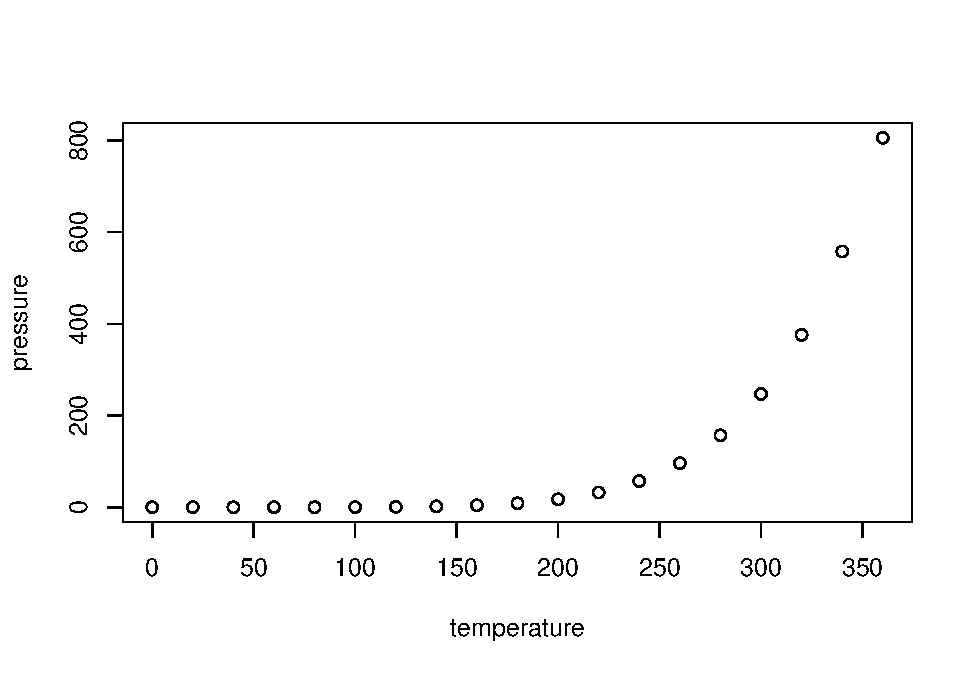
\includegraphics{4-Workshop_examples_files/figure-latex/pressure-1.pdf}
\caption{Figure of something at \(40^\circ 10^\prime\).
\label{fig:pressure}}
\end{figure}

<<<<<<< HEAD
=======
This is inline math mode for Latex \(40^\circ 10^\prime\)

>>>>>>> refs/remotes/melmonk/master
Note, you need extra \textbackslash{}s when using LaTeX syntax within an
R code chunk, or when inserting a backslash in R markdown. The same goes
with percent signs and any other LaTeX reserved symbol. You can use a \%
\(\%\)

We can now reference Figure \ref{fig:pressure}. Note where this text
ends up.

Note that the \texttt{echo\ =\ FALSE} parameter was added to the code
chunk to prevent printing of the R code that generated the plot.

\FloatBarrier

This is the LaTex inline math version (only one \textbackslash{}):
\(40^\circ 10^\prime\)

\FloatBarrier

We can now reference Figure \ref{fig:pressure}. Note where this text
ends up.

Note that the \texttt{echo = FALSE} parameter was added to the code
chunk to prevent printing of the R code that generated the plot.

\section{Tables}\label{tables}

\begin{table}[ht]
\centering
\caption{This is where you write your caption} 
\label{tab:Table_example}
\scalebox{0.7}{
\begin{tabular}{crcrcrcrcrc}
  \hline
Sample & Test1 & Test2 & Test3 & Test4 & Test5 & Test6 & Test7 & Test8 & Test9 & Test10 \\ 
  \hline
<<<<<<< HEAD
  1 & 333000000000.00 & 97.00 &  45 & 7169 & 5656 & 2642 & 8534 & 9173.00 & 230 & 2733 \\ 
    3 & 345.00 & 976.00 &   6 & 105 & 6382 & 2277 & 5848 & 7339495403.00 & 8613 & 5025 \\ 
    5 & 34.00 & 3333333333.00 &   7 & 2395 & 5632 & 5542 & 1645 & 380.00 & 1263 & 6728 \\ 
    7 & 234.00 & 34.00 &  46 & 5619 & 6063 & 8973 & 9362 & 1870.00 & 7651 & 683 \\ 
    9 & 234.00 & 0.00 &  45 & 6531 & 6824 & 3609 & 7627 & 3363.00 & 1534 & 8333 \\ 
   \hline
\end{tabular}
}
\end{table}

\begin{table}[ht]
\centering
\caption{WA black rockfish sensitivity table} 
\label{tab:Table_brfWA}
\scalebox{0.35}{
\begin{tabular}{lllllllllllllllllllll}
  \hline
X & X.1 & X.2 & X.3 & X.4 & X.5 & X.6 & X.7 & X.8 & X.9 & X.10 & X.11 & X.12 & X.13 & X.14 & X.15 & X.16 & X.17 & X.18 & X.19 & X.20 \\ 
  \hline
 & Sensitivity scenario &  &  &  &  &  &  &  &  &  &  &  &  &  &  &  &  &  &  &  \\ 
   & Base case &  & Index removal &  &  &  &  & Length comp removal &  &  &  &  &  &  &  & Age Comp removal &  &  &  &  \\ 
   &  &  & 1 & 2 & 3 & 4 &  & 5 & 6 & 7 & 8 & 9 & 20 & 11 &  & 12 & 13 & 14 & 15 & 16 \\ 
  Total Likelihood & 1213 &  & 1214 & 1224 & 1208 & 1217 &  & 1071 & 1100 & 1180 & 1149 & 1176 & 1191 & 814 &  & 955 & 1090 & 993 & 865 & 298 \\ 
  Survey Likelihood Components &  &  &  &  &  &  &  &  &  &  &  &  &  &  &  &  &  &  &  &  \\ 
  Onboard CPUE & -1.23 &  & -0.22 & -1.50 & -2.01 & -1.77 &  & -0.68 & -2.57 & -1.31 & 0.50 & -3.38 & -1.00 & -3.34 &  & -1.25 & -1.27 & -0.92 & -2.98 & -0.97 \\ 
  Onboard CPUE II & -14.28 &  & -14.30 & -2.61 & -13.84 & 49.95 &  & -13.63 & -14.34 & -14.14 & -17.54 & -17.68 & -14.69 & -17.32 &  & -14.35 & -14.30 & -15.22 & -14.72 & -10.99 \\ 
  Dockside & 1.38 &  & 0.06 & 3.19 & 7.84 & 13.86 &  & -3.94 & 1.24 & 2.57 & -2.17 & 1.05 & 0.43 & -8.84 &  & 0.96 & 1.45 & 0.39 & 10.02 & -4.15 \\ 
  Length Likelihood Components &  &  &  &  &  &  &  &  &  &  &  &  &  &  &  &  &  &  &  &  \\ 
  Trawl & 121.25 &  & 121.54 & 121.66 & 118.82 & 118.50 &  & 348.68 & 119.55 & 121.38 & 114.58 & 120.54 & 120.84 & 1052.56 &  & 121.03 & 117.73 & 122.25 & 119.43 & 110.18 \\ 
  Non-trawl dead & 104.24 &  & 103.66 & 103.58 & 104.31 & 103.15 &  & 111.66 & 398.19 & 103.91 & 100.45 & 102.75 & 104.27 & 673.91 &  & 97.83 & 105.41 & 104.46 & 106.17 & 97.44 \\ 
  Non-trawl live & 30.50 &  & 30.70 & 30.34 & 30.56 & 30.48 &  & 30.77 & 29.75 & 417.64 & 31.83 & 31.49 & 30.32 & 361.16 &  & 30.30 & 30.69 & 30.16 & 30.74 & 30.09 \\ 
  Recreational & 46.83 &  & 48.00 & 45.75 & 44.09 & 41.41 &  & 40.62 & 44.20 & 47.04 & 921.14 & 48.52 & 48.97 & 853.58 &  & 44.85 & 47.82 & 46.46 & 41.98 & 32.47 \\ 
  Onboard CPUE & 28.92 &  & 28.76 & 28.57 & 29.36 & 29.30 &  & 27.65 & 27.52 & 28.85 & 33.27 & 213.61 & 29.22 & 129.44 &  & 29.06 & 28.96 & 28.70 & 29.01 & 27.87 \\ 
  Recreational research & 21.31 &  & 21.59 & 21.45 & 20.16 & 19.81 &  & 21.02 & 21.34 & 20.76 & 26.24 & 20.53 & 24.30 & 32.50 &  & 20.76 & 21.34 & 21.34 & 20.68 & 19.19 \\ 
  Age Likelihood Components &  &  &  &  &  &  &  &  &  &  &  &  &  &  &  &  &  &  &  &  \\ 
  Trawl & 228.27 &  & 228.31 & 228.04 & 228.37 & 228.46 &  & 223.88 & 225.82 & 227.90 & 225.23 & 227.29 & 228.02 & 223.95 &  & 342.49 & 220.50 & 226.16 & 212.04 & 725.40 \\ 
  Non-trawl dead & 118.52 &  & 118.49 & 118.55 & 118.61 & 118.49 &  & 116.75 & 119.54 & 118.70 & 120.62 & 118.33 & 118.47 & 116.30 &  & 102.42 & 129.04 & 117.55 & 125.23 & 98.74 \\ 
  Recreational & 212.60 &  & 212.92 & 212.45 & 211.78 & 211.50 &  & 212.44 & 213.10 & 212.07 & 211.88 & 211.29 & 212.51 & 211.45 &  & 216.24 & 211.79 & 228.94 & 193.87 & 337.53 \\ 
  Recreational research & 316.66 &  & 315.27 & 316.94 & 319.89 & 319.92 &  & 308.24 & 317.69 & 314.47 & 304.63 & 316.61 & 315.79 & 290.14 &  & 309.60 & 320.79 & 313.41 & 484.47 & 515.43 \\ 
  Parameters &  &  &  &  &  &  &  &  &  &  &  &  &  &  &  &  &  &  &  &  \\ 
  NatM\_p\_1\_Fem\_GP\_1 & 0.18 &  & 0.19 & 0.18 & 0.17 & 0.16 &  & 0.22 & 0.19 & 0.18 & 0.16 & 0.18 & 0.18 & 0.36 &  & 0.16 & 0.19 & 0.18 & 0.17 & 0.16 \\ 
  L\_at\_Amin\_Fem\_GP\_1 & 23.39 &  & 23.42 & 23.44 & 23.35 & 23.44 &  & 23.23 & 23.36 & 23.35 & 23.49 & 23.29 & 23.37 & 23.29 &  & 24.08 & 23.36 & 24.22 & 19.50 & 28.87 \\ 
  L\_at\_Amax\_Fem\_GP\_1 & 54.54 &  & 54.56 & 54.62 & 54.41 & 54.46 &  & 53.72 & 55.46 & 54.54 & 54.58 & 54.35 & 54.54 & 50.77 &  & 53.06 & 55.42 & 54.91 & 52.99 & 53.28 \\ 
  VonBert\_K\_Fem\_GP\_1 & 0.15 &  & 0.15 & 0.15 & 0.15 & 0.15 &  & 0.15 & 0.14 & 0.15 & 0.15 & 0.16 & 0.15 & 0.16 &  & 0.15 & 0.15 & 0.14 & 0.23 & 0.09 \\ 
  CV\_young\_Fem\_GP\_1 & 0.09 &  & 0.09 & 0.09 & 0.09 & 0.09 &  & 0.09 & 0.10 & 0.09 & 0.10 & 0.09 & 0.09 & 0.10 &  & 0.09 & 0.10 & 0.11 & 0.05 & 0.07 \\ 
  CV\_old\_Fem\_GP\_1 & 0.07 &  & 0.07 & 0.07 & 0.07 & 0.07 &  & 0.07 & 0.07 & 0.07 & 0.07 & 0.07 & 0.07 & 0.06 &  & 0.06 & 0.06 & 0.07 & 0.08 & 0.03 \\ 
  NatM\_p\_1\_Mal\_GP\_1 & 0.13 &  & 0.13 & 0.13 & 0.12 & 0.11 &  & 0.14 & 0.14 & 0.13 & 0.11 & 0.13 & 0.13 & 0.16 &  & 0.12 & 0.14 & 0.13 & 0.13 & 0.13 \\ 
  L\_at\_Amin\_Mal\_GP\_1 & 25.21 &  & 25.24 & 25.21 & 25.12 & 25.08 &  & 25.07 & 25.32 & 25.11 & 24.89 & 24.89 & 25.14 & 24.70 &  & 25.81 & 25.12 & 25.62 & 23.55 & 25.32 \\ 
  L\_at\_Amax\_Mal\_GP\_1 & 46.00 &  & 45.96 & 46.01 & 46.02 & 46.06 &  & 45.44 & 46.24 & 46.04 & 46.10 & 45.86 & 45.98 & 43.62 &  & 45.88 & 46.43 & 45.43 & 46.87 & 47.30 \\ 
  VonBert\_K\_Mal\_GP\_1 & 0.21 &  & 0.21 & 0.21 & 0.22 & 0.22 &  & 0.21 & 0.20 & 0.22 & 0.23 & 0.22 & 0.22 & 0.25 &  & 0.19 & 0.21 & 0.21 & 0.24 & 0.13 \\ 
  CV\_young\_Mal\_GP\_1 & 0.09 &  & 0.09 & 0.09 & 0.10 & 0.09 &  & 0.10 & 0.09 & 0.10 & 0.10 & 0.10 & 0.10 & 0.11 &  & 0.09 & 0.10 & 0.10 & 0.05 & 0.06 \\ 
  CV\_old\_Mal\_GP\_1 & 0.07 &  & 0.07 & 0.07 & 0.07 & 0.07 &  & 0.07 & 0.07 & 0.07 & 0.07 & 0.07 & 0.07 & 0.04 &  & 0.06 & 0.07 & 0.08 & 0.07 & 0.04 \\ 
  SR\_LN(R0) & 7.61 &  & 7.66 & 7.52 & 7.46 & 7.23 &  & 7.88 & 7.71 & 7.58 & 7.36 & 7.60 & 7.64 & 8.22 &  & 7.54 & 7.64 & 7.63 & 7.56 & 7.70 \\ 
  SizeSel\_1P\_1\_Trawl & 49.34 &  & 49.34 & 49.31 & 49.47 & 49.48 &  & 39.01 & 48.84 & 49.38 & 49.82 & 49.48 & 49.38 & 17.02 &  & 49.80 & 49.36 & 49.23 & 49.03 & 49.66 \\ 
  SizeSel\_1P\_2\_Trawl & 0.32 &  & 0.32 & 0.33 & 0.29 & 0.27 &  & 2.41 & 0.10 & 0.31 & 0.06 & 0.31 & 0.30 & -3.45 &  & 0.29 & 0.40 & 0.28 & 0.40 & 0.27 \\ 
  SizeSel\_1P\_3\_Trawl & 3.47 &  & 3.47 & 3.46 & 3.49 & 3.49 &  & -0.62 & 3.41 & 3.48 & 3.57 & 3.49 & 3.48 & -0.44 &  & 3.65 & 3.48 & 3.43 & 3.57 & 3.70 \\ 
  SizeSel\_2P\_1\_nonTrawldead & 41.72 &  & 41.68 & 41.75 & 41.83 & 41.87 &  & 42.97 & 25.01 & 41.72 & 41.00 & 41.26 & 41.57 & 36.38 &  & 41.90 & 41.53 & 42.07 & 41.56 & 42.83 \\ 
  SizeSel\_2P\_2\_nonTrawldead & -1.82 &  & -1.83 & -1.83 & -1.79 & -1.82 &  & -1.17 & -0.63 & -1.77 & -5.82 & -2.36 & -1.86 & -2.30 &  & -2.20 & -2.14 & -1.80 & -1.78 & -5.83 \\ 
  SizeSel\_2P\_3\_nonTrawldead & 4.28 &  & 4.27 & 4.29 & 4.29 & 4.30 &  & 4.34 & -0.72 & 4.28 & 4.31 & 4.28 & 4.27 & -1.59 &  & 4.31 & 4.26 & 4.31 & 4.27 & 4.37 \\ 
  SizeSel\_3P\_1\_nonTrawllive & 34.58 &  & 34.54 & 34.57 & 34.68 & 34.69 &  & 34.86 & 34.83 & 35.00 & 34.21 & 34.46 & 34.53 & 34.63 &  & 34.78 & 34.60 & 34.74 & 34.49 & 35.95 \\ 
  SizeSel\_3P\_2\_nonTrawllive & -0.98 &  & -1.06 & -1.10 & -0.88 & -1.29 &  & -0.31 & -0.90 & -3.90 & -8.12 & -2.03 & -1.16 & -2.14 &  & -0.43 & -1.28 & -0.50 & -0.35 & -0.39 \\ 
  SizeSel\_3P\_3\_nonTrawllive & 2.79 &  & 2.78 & 2.79 & 2.80 & 2.81 &  & 2.84 & 2.83 & -0.90 & 2.72 & 2.74 & 2.78 & -1.01 &  & 2.85 & 2.78 & 2.84 & 2.72 & 3.19 \\ 
  SizeSel\_3P\_4\_nonTrawllive & 4.15 &  & 4.30 & 4.34 & 4.01 & 4.60 &  & 2.46 & 3.84 & -1.03 & 5.22 & 5.12 & 4.43 & -1.01 &  & 2.39 & 4.48 & 2.87 & 2.20 & 1.81 \\ 
  SizeSel\_3P\_6\_nonTrawllive & -3.17 &  & -3.82 & -3.99 & -2.47 & -3.63 &  & -0.68 & -3.06 & -4.99 & -4.73 & -4.70 & -4.16 & -4.96 &  & -0.79 & -4.31 & -1.47 & -0.90 & -0.12 \\ 
  SizeSel\_4P\_1\_Rec & 31.24 &  & 31.21 & 31.12 & 31.42 & 31.38 &  & 31.62 & 31.37 & 31.33 & 35.00 & 31.07 & 31.20 & 35.49 &  & 31.18 & 31.23 & 31.17 & 31.26 & 31.19 \\ 
  SizeSel\_4P\_2\_Rec & -3.05 &  & -3.03 & -2.99 & -3.26 & -3.22 &  & -3.92 & -2.93 & -3.07 & 2.73 & -3.11 & -2.99 & -1.85 &  & -2.94 & -2.98 & -3.17 & -3.51 & -3.52 \\ 
  SizeSel\_4P\_3\_Rec & 3.35 &  & 3.35 & 3.35 & 3.36 & 3.37 &  & 3.39 & 3.36 & 3.35 & -0.60 & 3.35 & 3.35 & -0.30 &  & 3.38 & 3.34 & 3.34 & 3.26 & 3.46 \\ 
  SizeSel\_5P\_1\_OnboardCPUE & 26.89 &  & 26.74 & 26.47 & 26.91 & 26.31 &  & 27.33 & 26.81 & 26.95 & 26.36 & 31.00 & 26.77 & 44.90 &  & 26.49 & 26.90 & 26.69 & 27.28 & 26.70 \\ 
  SizeSel\_5P\_2\_OnboardCPUE & -2.12 &  & -2.10 & -2.11 & -2.09 & -2.03 &  & -2.33 & -2.07 & -2.13 & -2.05 & -4.84 & -2.11 & -4.08 &  & -2.03 & -2.13 & -2.12 & -2.17 & -2.19 \\ 
  SizeSel\_5P\_3\_OnboardCPUE & 2.28 &  & 2.22 & 2.20 & 2.28 & 2.15 &  & 2.41 & 2.21 & 2.32 & 2.07 & -0.92 & 2.23 & -3.99 &  & 2.11 & 2.27 & 2.12 & 2.44 & 2.29 \\ 
  SizeSel\_7P\_1\_RecResearch & 26.33 &  & 26.34 & 25.83 & 26.47 & 25.78 &  & 28.99 & 26.76 & 26.44 & 25.02 & 25.67 & 32.50 & 32.50 &  & 26.41 & 26.41 & 26.74 & 28.36 & 26.75 \\ 
  SizeSel\_7P\_2\_RecResearch & -1.44 &  & -1.44 & -1.37 & -1.46 & -1.36 &  & -2.06 & -1.50 & -1.45 & -1.23 & -1.34 & 0.00 & 0.00 &  & -1.46 & -1.45 & -1.52 & -1.84 & -1.56 \\ 
  SizeSel\_7P\_3\_RecResearch & 2.89 &  & 2.89 & 2.73 & 2.93 & 2.73 &  & 3.66 & 2.99 & 2.92 & 2.44 & 2.66 & 4.00 & 4.00 &  & 2.96 & 2.92 & 3.05 & 3.47 & 3.35 \\ 
  Catchability (analytic solution) &  &  &  &  &  &  &  &  &  &  &  &  &  &  &  &  &  &  &  &  \\ 
  Onboard CPUE & 8.20E-05 &  & 7.63E-05 & 8.49E-05 & 9.67E-05 & 1.07E-04 &  & 6.84E-05 & 7.83E-05 & 8.58E-05 & 7.12E-05 & 1.10E-04 & 7.84E-05 & 1.30E-03 &  & 7.93E-05 & 8.23E-05 & 7.75E-05 & 1.27E-04 & 6.18E-05 \\ 
  Onboard CPUE II & 9.39E-05 &  & 8.51E-05 & 1.19E-04 & 1.29E-04 & 2.54E-04 &  & 7.94E-05 & 8.49E-05 & 1.02E-04 & 8.57E-05 & 1.18E-04 & 8.85E-05 & 1.19E-03 &  & 9.09E-05 & 9.42E-05 & 8.86E-05 & 1.57E-04 & 6.81E-05 \\ 
  Dockside & 4.87E-05 &  & 4.52E-05 & 5.12E-05 & 5.83E-05 & 6.72E-05 &  & 4.19E-05 & 4.47E-05 & 5.13E-05 & 4.37E-05 & 6.16E-05 & 4.64E-05 & 7.97E-04 &  & 4.77E-05 & 4.88E-05 & 4.60E-05 & 7.51E-05 & 3.76E-05 \\ 
  Dervied quantities &  &  &  &  &  &  &  &  &  &  &  &  &  &  &  &  &  &  &  &  \\ 
  SB0 & 1062 &  & 1045 & 1012 & 1070 & 1046 &  & 726 & 1104 & 1067 & 1222 & 1047 & 1055 & 105 &  & 1214 & 1037 & 1038 & 1164 & 1387 \\ 
  SB2015 & 353 &  & 392 & 249 & 229 & 55 &  & 287 & 398 & 320 & 469 & 410 & 378 & 49 &  & 353 & 357 & 363 & 222 & 406 \\ 
  SB2015/SB0 & 33\% &  & 38\% & 25\% & 21\% & 5\% &  & 40\% & 36\% & 30\% & 38\% & 39\% & 36\% & 46\% &  & 29\% & 34\% & 35\% & 19\% & 29\% \\ 
  Yield at SPR50\% & 319 &  & 325 & 299 & 300 & 265 &  & 336 & 326 & 314 & 321 & 319 & 324 & 373 &  & 320 & 318 & 318 & 335 & 319 \\ 
=======
1 & 333000000000 & 97 & 45 & 7169 & 5656 & 2642 & 8534 & 9173 & 230 & 2733 \\ 
  3 & 345 & 976 & 6 & 105 & 6382 & 2277 & 5848 & 7339495403 & 8613 & 5025 \\ 
  5 & 34 & 3333333333 & 7 & 2395 & 5632 & 5542 & 1645 & 380 & 1263 & 6728 \\ 
  7 & 234 & 34 & 46 & 5619 & 6063 & 8973 & 9362 & 1870 & 7651 & 683 \\ 
  9 & 234 & 0 & 45 & 6531 & 6824 & 3609 & 7627 & 3363 & 1534 & 8333 \\ 
>>>>>>> refs/remotes/melmonk/master
   \hline
\end{tabular}
}
\end{table}

Try changing the R chunk options above.

We can now reference Table \ref{tab:Table_example}.

Now, try putting the R code chunk within and HTML comment.

\section{Create you own table}\label{create-you-own-table}

Either create a .csv file or copy one into the repo folder on your
computer.

Now, create a table!

\section{Math mode}\label{math-mode}

You can use LaTeX math mode both inline and for inserting equations.
It's handy for using inline math mode for management measure and
lat/long.

<<<<<<< HEAD
Inline looks like this: \(SPR_{40\%}\)\\*Note the \% sign has a ~when
used in math mode, but not in R markdown text.
=======
Inline looks like this: \(SPR_{40\%}\)\\
*Note the \% sign has a ~when used in math mode, but not in R markdown
text.
>>>>>>> refs/remotes/melmonk/master

To get degrees and minutes type: \(40^\circ 10^\prime\)

\section*{References}\label{references}
\addcontentsline{toc}{section}{References}

Love, M., Yoklavich, M., and Thorsteinson, L. 2002. The rockfishes of
the northeast Pacific. University of California Press, Berkeley, CA,
USA.

\end{document}
